 \documentclass[12pt, a4paper, american]{article}
\usepackage[a4paper]{geometry}
%\newgeometry{left=1in, bottom=1in, top=1in, right=1in}
%\newgeometry{left=1.25in, bottom=1.25in, top=1.25in, right=1.25in}
\renewcommand{\baselinestretch}{1.5}
\usepackage{amsmath,a4,babel,booktabs,graphicx,rotating,float,amsfonts,mathtools, amsthm, amssymb}
\usepackage[LGR,T1]{fontenc} % spell out all text encodings used
\usepackage[utf8]{inputenc} %
\usepackage{caption}
\usepackage{subcaption} % for subfigures 
\usepackage{graphicx, mathptmx}
%\usepackage[position=top]{subfig}
\usepackage[sort&compress]{natbib}

\usepackage[plain]{fancyref} %fancy references
\usepackage{microtype,framed} %other packages added
\usepackage{wasysym}
\usepackage{multirow,array}
\usepackage{multicol}
\usepackage{tcolorbox} % to create colored text boxes
\usepackage{bbm}
\usepackage{graphicx}
\usepackage{enumitem} 
\usepackage{xcolor}
\usepackage{abbrevs}
\usepackage{pgffor}
\usepackage{comment}
\usepackage{nicefrac}
\setlength{\parskip}{5pt}
\usepackage{setspace}
\usepackage{titling}
\onehalfspacing 
\usepackage{pdflscape}
\usepackage{threeparttable}
\usepackage{soul}
\usepackage{clipboard}
\newclipboard{myclipboard}
\usepackage[citecolor= black,
			colorlinks=true,
		    linkcolor = black,
            urlcolor  = black]{hyperref}
\usepackage{xurl}
\usepackage{chngcntr}   % for per-chapter numbering of figures
\usepackage{float}



\newenvironment{q}%for the appendix
{
\setlength{\parindent}{0pt}
}
%
\makeatletter
\usepackage{tikz}
\usepackage{verbatim}
\usetikzlibrary{positioning, shapes, arrows, fit, backgrounds}
\newcommand*{\h}{\hspace{5pt}}% for indentation
\usepackage{epigraph} % for nice quote 
\usepackage{makecell} % for nice table cells

\newcommand{\ssection}[1]{\section[#1]{\centering #1}}

\newgeometry{top=2.2cm, bottom=2.2cm, left=2.2cm, right=2.2cm}

% ------------ Mathematical environments -----------

\theoremstyle{plain}
\newtheorem{theorem}{Theorem}

\theoremstyle{definition}
\newtheorem{prediction}[theorem]{Prediction}


% *****************************************************************
% Estout related things
% *****************************************************************
\newcommand{\sym}[1]{\rlap{#1}}% Thanks to David Carlisle

\let\estinput=\input% define a new input command so that we can still flatten the document

\newcommand{\estwide}[3]{
		\vspace{.75ex}{
			\begin{tabular*}
			{\textwidth}{@{\hskip\tabcolsep\extracolsep\fill}l*{#2}{#3}}
			\toprule
			\estinput{#1}
			\bottomrule
			\addlinespace[2.50ex]
			\end{tabular*}
			}
		}	

\newcommand{\estauto}[3]{
		\vspace{.75ex}{
			\begin{tabular}{l*{#2}{#3}}
			\toprule
			\estinput{#1}
			\bottomrule
			\addlinespace[2.75ex]
			\end{tabular}
			}
		}

% Allow line breaks with \\ in specialcells
	\newcommand{\specialcell}[2][c]{%
	\begin{tabular}[#1]{@{}c@{}}#2\end{tabular}}


%% For quote

\makeatletter
\newenvironment{chapquote}[2][3em]
  {\setlength{\@tempdima}{#1}%
   \def\chapquote@author{#2}%
   \parshape 1 \@tempdima \dimexpr\textwidth-2\@tempdima\relax%
   \itshape}
  {\par\normalfont\hfill--\ \chapquote@author\hspace*{\@tempdima}\par\bigskip}
\makeatother

% *****************************************************************


% *****************************************************************
% Custom subcaptions
% *****************************************************************
% Note/Source/Text after Tables

% Note/Source/Text after Tables
\newcommand{\tabtext}[1]{%
	\vspace{-0.5ex}
 \begin{tablenotes}[para,flushleft]
 \hspace{5pt}
 \hangindent=1.75em
 #1
 \end{tablenotes}
}

\newcommand{\tabnote}[1]{\parbox{\linewidth}{\tabtext{\emph{Note:~}~#1}}}
\newcommand{\tabsource}[1]{\tabtext{\emph{Source:~}~#1}}
\newcommand{\starnote}{\vspace{0.75ex}\tabtext{* $p$\;<\;0.10, ** $p$\;<\;0.05, *** $p$\;<\;0.01. Robust standard errors in parentheses.}}
\newcommand{\starnotebootstrap}{\vspace{0.75ex}\tabtext{* $p$\;<\;0.10, ** $p$\;<\;0.05, *** $p$\;<\;0.01. Bootstrapped standard errors in parentheses.}}

\newcommand{\starnotesimple}{\vspace{0.75ex}\tabtext{* $p$\;<\;0.10, ** $p$\;<\;0.05, *** $p$\;<\;0.01.}}

\newcommand{\starnotenonrobust}{\tabtext{* $p$\;<\;0.10, ** $p$\;<\;0.05, *** $p$\;<\;0.01. Standard errors in parentheses.}}

% *****************************************************************
% Custom subcaptions: Figure
% *****************************************************************
% Note/Source/Text after Tables
\newcommand{\figtext}[1]{
	\vspace{-0.5ex}
	\captionsetup{justification=justified,font=small}
	\caption*{\hspace{8pt}\hangindent=1.5em #1}
	}
%\newcommand{\fignote}[1]{\figtext{\scriptsize Notes:~#1}}
\newcommand{\fignote}[1]{\figtext{\emph{Note:~}~#1}}

\newcommand{\figsource}[1]{\figtext{\emph{Source:~}~#1}}

% Character substitution that prints brackets and the minus symbol in text mode and does not reserve any space. Thanks to David Carlisle
\def\yyy{%
  \bgroup\uccode`\~\expandafter`\string-%
  \uppercase{\egroup\edef~{\noexpand\text{\llap{\textendash}\relax}}}%
  \mathcode\expandafter`\string-"8000 }

\def\xxxl#1{%
\bgroup\uccode`\~\expandafter`\string#1%
\uppercase{\egroup\edef~{\noexpand\text{\noexpand\llap{\string#1}}}}%
\mathcode\expandafter`\string#1"8000 }

\def\xxxr#1{%
\bgroup\uccode`\~\expandafter`\string#1%
\uppercase{\egroup\edef~{\noexpand\text{\noexpand\rlap{\string#1}}}}%
\mathcode\expandafter`\string#1"8000 }
\def\textsymbols{\xxxl[\xxxr]\xxxl(\xxxr)\yyy}

% *****************************************************************
% siunitx
% *****************************************************************
\usepackage{siunitx} % centering in tables
	\sisetup{
		detect-mode,
		tight-spacing		= true,
		group-digits		= false ,
		input-signs		= ,
		input-symbols		= ( ) [ ] - + *,
		input-open-uncertainty	= ,
		input-close-uncertainty	= ,
		table-align-text-post	= false
        }

\usepackage{footmisc} %NR: Changed this to use numeric footnotes again
\DefineFNsymbolsTM{myfnsymbols}{% def. from footmisc.sty "bringhurst" symbols
  \textasteriskcentered *
  \textdagger    \dagger
  \textdaggerdbl \ddagger
  \textsection   \mathsectionwe 
%  \textbardbl    \|%
%  \textparagraph \mathparagraph
}%
\setfnsymbol{myfnsymbols}



\theoremstyle{definition}
\newtheorem{prop}[theorem]{Proposition}
\newtheorem{corollary}[theorem]{Corollary}
%\newtheorem{prediction}[theorem]{Prediction}
\newtheorem{hypothesis}[theorem]{Hypothesis}

\newtheorem{result}{Result}



% ----------------------- Abbreviations ----------------------------------

% General abbreviations
\newcommand{\lucid}{Lucid}
\newcommand{\fox}{\textit{Fox News}}
\newcommand{\msnbc}{\textit{MSNBC}}
\newcommand{\bidenrescueplan}{\textit{Biden Rescue Plan}}
\newcommand{\americanrescueplan}{\textit{American Rescue Plan}}

\newcommand{\onlineappendix}{Online Appendix}

% Statistical abbreviations
\newcommand{\n}{$n$\;=\;}
\newcommand\onestar{$p$\;<\;0.10}
\newcommand\twostar{$p$\;<\;0.05}
\newcommand\threestar{$p$\;<\;0.01}
\newcommand\nostar{$p$\;>\;0.10}
\newcommand\pt{$p$\;<\;0.001}
\newcommand{\p}{$p$\;=\;}

% Experiment Instructions
\newcommand{\includeInstructions}[1]{
	\begin{center}
		\includegraphics[width=0.90\textwidth]{#1.png}
	\end{center}
}


\newcommand{\includeInstructionsLong}[1]{
	\begin{center}
		\includegraphics[height=0.95\textheight]{#1.png}
	\end{center}
}










\title{\textsc{Time and Information in Bargaining}}
\author{Dongkyu Chang \;\; Peter Cramton \;\; Jeongbin Kim \\ \;\;Axel Ockenfels \;\; Nicolas Roever }





\date{\today}


\begin{document}

\maketitle
\setcounter{page}{0}
\thispagestyle{empty}

\begin{abstract}
\noindent We analyse bilateral bargaining when negotiating itself is costly and delay destroys surplus under different information structures.  
First, we embed \emph{per--second transaction costs} and exponential discounting into a continuous-time Rubinstein–Cramton framework with one–sided and two-sided incomplete information.  The equilibrium for one-sided uncertainty is characterised by two endogenous cut-offs that split buyer types into (i) immediate terminators, (ii) delay-and-signal types, and (iii) immediate accepters; closed-form comparative statics show that higher costs or lower discount rates compress the delay region.  
Second, we test the theory in a \(2\times2\) laboratory experiment (\(N=384\)) that independently varies information structure (one- vs.\ two-sided private values) and transaction costs incurred during bargaining. 


\end{abstract}

\bigskip

\noindent{\small\textbf{Keywords}: Bargaining; Transaction costs; Delay; Information asymmetry; Laboratory experiment; First-mover advantage}\\
\noindent{\small\textbf{JEL codes}: C78; C91; C92; D82; D44}
\vspace{0.5em}
\vspace*{5cm}

\pagebreak


\section{Introduction}
Bargaining is omnipresent in our economic system and the theoretical literature has proposed a large stream of models to explain bargaining outcomes under various circumstances. 

\begin{comment}
    We find that intermediate and complete information reduce trade failures for small-surplus items. This is in line with a large experimental literature on one-sided (e.g. Forsythe et al., 1991; Cason and Reynolds, 2005; Camerer et al., 2019) and two-sided (e.g. Valley et al., 2002; Ellingsen et al., 2009) incomplete information bargaining.
\end{comment}

In this paper, we present a model which explicitly incorporates transaction costs---occurring because negotiating itself is costly---as well as costs of time delay, occurring because delaying an agreement is costly. We derive equilibrium results for one-sided incomplete information bargaining. \\

We then turn to the laboratory and collect data on a very unstructured negotation. We implement a 2x2 design, where we vary whether transaction costs exist or nor and we vary whether there is one-sided incomplete information (the asymetric case) and two-sided incomplete information. \\

Our data on one-sided incomplete infromation allows us to compare the existing models of bargaining---including our own---in a ``horse race''.

While we cannot derive a theoretical equilibrium for the case of two-sided incomplete information, our data allows characterize the empirical equilibrium. 



\paragraph{Related Literature}
We relate to a large literature stream proposing theoretical models for bilateral bargaining under incomplete information. Among theoretical work analysing one-sided incomplete information, \citep{rubinstein1985choice, bikhchandani1992theory, grossman1986perfect, gul1988delay, cramton_dynamic_1991} analyze structures where both agents can make offers. Our model is a more complete extension, as we consider transaction costs and costs of time delay simultaneously. \\
Among the literature on two-sided incomplete information \citep{chatterjee1987bargaining, cramton_strategic_1992, abreu2000bargaining, watson1998alternating}, we NOT SURE HERE. 
Our theoretical model is an extension of \citet{cramton_dynamic_1991} and \citet{cramton_strategic_1992}. In this paper, we present a model which explicitly incorporates transaction costs---occurring because negotiating itself is costly---as well as costs of time delay, occurring because delaying an agreement is costly. \\
@Dongkyu please expand this paragraph :). 
\\
We also relate to the literature studying bargaining behavior in the laboratory. Our setup allows for a ``horse race'' between the different theoretical models, as our environment closely matches the theoretical assumptions in the aforementioned literature.Our setup is among the few experiments which allow relatively unstructured bargaining. Our environment differs from \citet{bochet_beyond_2024}, as our subjects only trade on one good simultaneously. \\
\textcolor{red}{We need to expand this a lot} \\

This paper is organized as follows. \Fref{sec:model} develops the model, \Fref{sec:experimental_design} describes our experimental design and hypotheses and \Fref{sec:main_results} presents our main results. \Fref{sec:conclusion} concludes. 



\begin{comment}

Experiments on single-issue bargaining have documented extensively the relevance of behavioural factors such as fairness or strategic sophistication, see e.g. Roth (1995), Cooper and Kagel (2016), Fehr and Schmidt (1999), Bolton and Ockenfels (2000), Andreoni and Miller (2002), Embrey et al. (2015), Fanning and Kloosterman (2019) and Bochet and Siegenthaler (2021). Closely related to our work are Babcock et al. (1995), who document that an increased surplus can affect agreement rates negatively under complete information, and Huang et al. (2020), who show in an ultimatum bargaining context that fairness concerns are more pronounced when information is complete than when it is incomplete.
\end{comment}




\section{Model}
\label{sec:model}

\paragraph{Players and Types:} Consider a bilateral price negotiation. At the beginning of the negotiation, the buyer's and the seller's private types (values) $b\in[\underline B,\overline B]$ and $s\in[\underline S,\overline S]$ are drawn from probability distributions $F$ and $G$, respectively.
$F$ and $G$ are common knowledge, where they admit density functions $f$ and $g$, respectively. For any measurable $\mathcal{B}$, define $F(b|\mathcal{B})$ and $f(b|\mathcal{B})$ as the distribution and the density of $b$ conditional on $b\in\mathcal{B}$. Define $G(s|\mathcal{S})$ and $g(s|\mathcal{S})$ similarly for any measurable $\mathcal{S}$.


\paragraph{Bargaining Protocol:} The negotiation unfolds over an infinite horizon, where time is indexed by $t\in[0,\infty)$. After each player privately observes their own type, both players begin the negotiation at $t=0$ with ``silence.'' At every instant $t$, either party may choose ``break the silence.'' There are two ways of breaking silence. First, a party may make an initial price offer. If the two parties make initial offers at the same time, a fair coin is flipped to determine which offer stands as the initial offer. Second, a party may  break silence by terminating the negotiation.


After the initial offer, the following procedure repeats until either party accepts a standing offer or terminates the negotiation. 
    \begin{itemize}
    \item After a party makes an offer, the other has three possible responses: (1) a counteroffer, in which case the game continues, (2) acceptance, in which case trade occurs at the accepted price, or (3) termination, in which case the game ends without trade. 

    \item The response can occur anytime after the minimum time $t_0>0$ has passed. We are eventually interested in the limit $t_0\to 0$. 
    In the meantime, the party who has made the standing offer can also terminate the negotiation anytime after $t_0$ lapses. 
    \end{itemize}

\paragraph{Payoffs, Strategies and, Equilibrium:} 
If the players agree to trade at time $t$ for the price $p$,  the seller and buyer obtain the final payoffs 
    Recall that the seller's and the buyer's payoffs are given by 
    \begin{align}
    &u_S(s,t,p):=e^{-r_St}(p-s) - \int_0^t e^{-r_Sx} c_S \,\text{d}x
    =e^{-r_St}(p-s) - \frac{c_S}{r_S} (1-e^{-r_St}),\label{eq:utility_seller}
    \\
    &u_B(b,t,p):=e^{-r_Bt}(b-p) - \int_0^t e^{-r_Bx} c_B \,\text{d}x
    =e^{-r_Bt}(b-p) - \frac{c_B}{r_B} (1-e^{-r_Bt}).\label{eq:utility_buyer}
    \end{align}
where $r>0$ represents the common discounting rate, and $c_S>0$ and $c_B>0$ stand for each party's negotiation costs per unit of time during the negotiation. If the negotiation is terminated at time $t$, the seller and the buyer obtain 
    \begin{align*}
    &- \int_0^t e^{-rs} c_S \,\text{d}s = - \frac{c_S}{r} (1-e^{-rt})
    \quad\text{and}\quad- \int_0^t e^{-rs} c_B \,\text{d}s = - \frac{c_B}{r} (1-e^{-rt})
    \end{align*}
as their final payoffs. We will focus on pure-strategy Perfect Bayesian equilibrium (PBE). 

\section{Bargaining with Complete Information} \label{ss:complete_info}

As a benchmark, consider the case $b$ and $s$ are common knowledge, where $b\leq s$ is without loss. In equilibrium, the negotiation ends immediately with the following outcome: the seller and the buyer trade at a price $p^R(b,s)$, where the superscript $R$ stands for Rubinstein:
    \begin{align}\label{eq:rubinstine_price_00}
    p^R(b,s) \approx \left\{
    \begin{array}{cl}
    \frac{b+s}{2} - \frac{c_S-c_B}{2r} & \text{if $r(b-s)\geq|c_S-c_B|$,} 
    \\
    b  & \text{ if $r(b-s)< c_B-c_S$,}
    \\
    s & \text{ if $r(b-s)< c_S-c_B$.}
    \end{array}\right.
    \end{align}
Throughout the note, define 
    \begin{align*}
    &b^\diamondsuit :=\min\left\{\overline b, s+\frac{|c_S-c_B|}{r}\right\}
    \quad\text{and}\quad 
    s^\diamondsuit :=\min\left\{\underline s, b-\frac{|c_S-c_B|}{r}\right\}. 
    \end{align*}
    
\section{Bargaining with Buyer's Asymmetric Information}
\label{ss:one_sided_buyer}


Next, consider the case with one-sided asymmetric information such that (i) the seller's value $s$ is known and (ii) the seller believes that $b$ is drawn from the cumulative distribution $F(\cdot | [\underline b,\overline b])$, 
where $[\underline b, \overline b]\subset [\underline B, \overline B]$. We also impose $s\leq \underline b$ without loss; otherwise, all those types will terminate the negotiation at $t=0$ as there is no gain from trading.

\subsection{An Equilibrium}

 


\paragraph{Equilibrium play on the path:} 
The equilibrium play on the path is given as follows, where two cutoffs $b^*$ and $b^\dagger$ will be pinned down shortly. For any $t\geq 0$, $b$ and $\hat b$ such that $\underline b\leq b\leq \tilde b \leq\overline b$ define
    \begin{align}\label{eq:Delta}
    &\Delta (b|\hat b):= 
    \left\{
    \begin{array}{cl}\displaystyle
    0 & \forall b\in(\hat b, \overline b],
    \\[10pt]
    \displaystyle 
    \int_b^{\hat b} \frac{\partial p^R(z,s)/\partial z}{r[z-p^R(z,s)]+c_B}\text{d}z
	& \forall b\in[s\vee \underline b, \hat b]. 
    \end{array}\right.
  \end{align}

The seller begins by making an initial offer $p_0=p^R(b^*,s)$ at time $t=0$. Then:
	\begin{enumerate}[(i)]
	\item Each buyer type in $[b^*,\overline b]$ accepts the seller's initial offer $p^R(b^*,s)$ immediately.  
	\item Each buyer type in $[b^\dagger, b^*)$ (this interval is possibly empty) delays until $t=\Delta (b|b^*)$; in the meantime, the seller never terminates the negotiation. 
    In the continuation game after $t=\Delta (b|b^*)$, the seller holds the posterior belief $F(\cdot|{\Delta^{-1}(t|b^*)})$, and two players trade for the price $p^R(b,s)$ immediately.

  \item Each buyer type in $[\underline b, b^\dagger)$ (this interval is possibly empty) terminates the negotiation immediately (i.e., at time $t=t_0$). 
\end{enumerate}

On the path, each buyer type $b\in[b^\dagger,\overline b]$ earns
    \begin{align}\nonumber
    \widetilde v_B (b|b^*)=
    \left\{
    \begin{array}{ll}
    b-p^R(b^*,s) & \forall b\in(b^*, \overline b],
    \\[10pt]
    \displaystyle e^{-r\Delta (b|b^*)}\left[b-p^R(b, s)+\frac{c_B}{r}\right]-\frac{c_B}{r}  & \forall b\in[s\vee\underline b, b^*].
    \end{array}\right.
    \end{align}
Each $b\in[b^\dagger,b^*)$ must have no incentive to mimic each other.
Such incentive-compatibility condition, together with the ``boundary condition'' $\Delta (b^*|b^*)=0$, yields $\Delta (b|b^*)$ in \eqref{eq:Delta}.
For all buyer types with $\widetilde v_B (b;b^*)\leq 0$, it is profitable to terminate the negotiation immediately (without any delay). Thus, the cutoff type $b^\dagger$ must be as follows.
	\begin{align}\label{eq:b_ddagger}
	b^\dagger=b^\ddagger(b^*):=
    \left\{
    \begin{array}{cl}
    \sup \big\{b\in[s\vee \underline b, \overline b]: \widetilde v_B (b;b^*)\leq 0\big\} & \text{if $\widetilde v_B (s\vee \underline b|b^*)\leq 0$,}
    \\[5pt]
    s \vee \underline b & \text{if $\widetilde v_B (s\vee \underline b|b^*)> 0$.}
    \end{array}\right. 
	\end{align}
Note the tie-breaking rule here: The buyer terminates at $t=t_0\approx 0$ whenever $\widetilde v_B(b|b^*)=0$.


Next, we show that, at any time $t=\Delta (b|b^*)$, the seller is always willing to continue the negotiation for the next infinitesimal time $\text{d}t_\epsilon = \Delta (b-\epsilon|b^*)-\Delta (b|b^*)$. The seller's payoff from continuing the negotiation is at least 
	$$
	\pi_S(\epsilon|b):=\int_{b-\epsilon}^b 
	\left\{e^{-r[\Delta (z|b^*)-\Delta (b|b^*)]} \left(p^R(z,s)-s+\frac{c_S}{r}\right)-\frac{c_S}{r}\right\}
	\frac{f(z)}{F(b)-F(b^\dagger)}\text{d}z.
	$$
which converges to zero as $\epsilon\downarrow 0$. Note that 
	\begin{align*}
	\pi_S'(0^+|b) 
	=\lim_{\epsilon\to 0}\frac{\pi_S(\epsilon|b)}{\epsilon}
	=\frac{[p^R(b,s)-s]f(b)}{F(b)-F(b^\dagger)}\geq 0 
    \quad\forall b\geq s.
	\end{align*}
The inequality is strictly held whenever $p^R(b,s)>s$. 

\paragraph{Equilibrium play off the path:} Suppose that the seller offers the initial offer $\hat p_0$. Define 
    \begin{align*}
    \hat b :=& \left\{
    \begin{array}{cl}
    \overline b & \text{if $p^R(\overline b,s)<\hat p_0$,}
    \\
    \text{$b$ such that $\hat p_0=p^R(b,s)$} & \text{if $s<\hat p_0\leq p^R(\overline b,s)$,}
    \\
    s & \text{if $\hat p_0\leq s$. }
    \end{array}
    \right.
    \end{align*}
    % \begin{align*}
    % b^\ddagger(\hat b):= & \left\{
    % \begin{array}{cl}
    % \sup \big\{b\in[ s\vee \underline b, \overline b]: \widetilde v_B (b;\hat b)\leq 0\big\} & \text{if $\widetilde v_B (s\vee \underline b|\hat b)\leq 0$,}
    % \\
    % s \vee \underline b & \text{if $\widetilde v_B (s\vee \underline b|\hat b)> 0$.}
    % \end{array}\right. 
    % \end{align*}
In response to the seller's initial offer $\hat p_0$:
    \begin{enumerate}[(a)]
	\item Each $b\in [\hat b,\overline b]$ accepts the seller's initial offer $\hat p_0$ immediately.  
	\item Each $b\in[b^\ddagger(\hat b), \hat b)$ delays until $t=\Delta (b|\hat b)$; in the meantime, the seller never terminates the negotiation.  
    In the continuation game after $t=\Delta (b|\hat b)$, the seller holds the posterior belief $F(\cdot| \Delta^{-1}(t|\hat b))$, and two players trade for the price $p^R(b,s)$ immediately.
    \item Each $b\in[\underline b, b^\ddagger(\hat b))$ terminates the negotiation immediately (i.e., at time $t=t_0$). 
\end{enumerate}


If the buyer deviates from (a)--(c) by making a counteroffer at $t>\Delta (s\vee \underline b|\hat b)$, the seller holds the posterior belief that $b=s\vee\underline b$ with probability 1. This belief would induce the seller to terminate the negotiation immediately (i.e., at time $t+t_0$). 



\paragraph{Seller's Optimization Problem at $t=0$:}
At time $t=0$, the seller chooses a cutoff buyer type $\hat b$ and offers  $p_0=p^R(\hat b,s)$. Then, all buyer types $b\geq \hat b$ accepts it. Each buyer type lower than $\hat b$ either delays or terminates the negotiation, which results in the buyer's and the seller's payoffs $\widetilde V_B (b|\hat b)$ and $\widetilde V_S (b|\hat b)$, respectively:
	$$
	\widetilde V_S (b|b^*):=
	\left\{
	\begin{array}{ll}
    \displaystyle p^R(b^*,s)-s & \text{if $b\in[b^*,\overline b]$}
    \\[5pt]
	\displaystyle e^{-r\Delta (b|b^*)}\left(p^R(b,s)-s+\frac{c_S}{r}\right)-\frac{c_S}{r} & \text{if $b\in [b^\dagger, b^*)=[b^\ddagger(b^*), b^*)$}
	\\[5pt]
	0 & \text{if $b<b^\dagger=b^\ddagger(b^*)$} 
	\end{array}
	\right.
	$$
	$$
	\widetilde V_B (b|b^*):=\left\{
	\begin{array}{ll}
    \displaystyle b-p^R(b^*,s)& \text{if $b\in[b^*,\overline b]$}
    \\[5pt]
	\displaystyle e^{-r\Delta (b|b^*)}\left(b-p^R(b,s)+\frac{c_B}{r}\right)-\frac{c_B}{r} & \text{if $b\in [b^\dagger, b^*)=[b^\ddagger(b^*), b^*)$}
	\\[5pt]
	0 & \text{if $b<b^\dagger=b^\ddagger(b^*)$} 
	\end{array}
	\right.
	$$
On the path, the optimal cutoff $\hat b=b^*$ solves the following problem. 
	\begin{align}\label{eq:seller_optimization_problem}
	V_S (s|\underline b,\overline b
	)=\max_{b\in[s\vee \underline b,\overline b]}& \frac{F(\overline b)-F(b)}{F(\overline b)-F(\underline b)}(p^R(b,s)-s)
    +\int_{b^\ddagger(b)}^b \widetilde V_S (z|b)\frac{\text{d}F(z)}{F(\overline b)-F(\underline b)},
	\end{align}
where $b^\ddagger(\cdot)$ is given by \eqref{eq:b_ddagger}. 


\section{Uniform Symmetric Example}

Fix $s\leq \underline b < \overline b$, and suppose that the seller's prior belief is uniform over $[\underline b,\overline b]$, {\color{red} where $\underline b=0$}. Note that $\underline b$ implies $\underline b\vee s =s$. Furthermore, two players have the same negotiation cost $c=c_S=c_B$. {\color{red} Define $\kappa:=c/r$ as the ratio between negotiation cost and discounting rate.}

\subsection{Equilibrium}
With $c_B=c_S$, we have $b^\diamondsuit=s$, and thus, 
$p^R(b,s) = ({b+s})/{2}$ for all  $b$. By direct calculation  
    \begin{align*}
    &e^{-r\Delta (b|b^*)}
    % = \exp\left\{-r\int_b^{b^*} \frac{\partial p^R(z,s)/\partial z}{r[z-p^R(z,s)]+c_B}\text{d}z\right\}
    =\frac{r(b-s)+{\color{red} 2c_B}}{r(b^*-s)+{2c_B}}=\frac{b-s+2\kappa}{b^*-s+2\kappa},
    \\
   &
    \Delta(b|b^*) = \frac{1}{r} \ln \left[\frac{b-s+2\kappa}{b^*-s+2\kappa}\right]
    \\
    &\widetilde V_S (b|b^*)=\widetilde V_B (b|b^*)=\frac{1}{2}\frac{(b-s+2\kappa)^2}{{b^*}-s+2\kappa}-\kappa \quad\forall b\in[b^\dagger, b^*),
    \end{align*}
For the future reference, we compute
	$$
	b^\ddagger(\beta;b):=
    \sup\left\{
	{b\in[s\vee \underline b, \overline b]}:\, 
    \widetilde v_B (b;b)\leq \beta \right\} 
    $$
for any relevant $\beta\geq 0$, where $b^\ddagger(\beta;b):=s\vee \underline b$ for the case where $\widetilde v_B (s \vee \underline b;b)> \beta$. We can obtain $b^\ddagger(b)=b^\ddagger(0;b)$ as a special case. It is useful to define 
    $$
    D(\beta;b):=2(c_B+r\beta)[r(b-s)+c_S+c_B].
    $$
By direct calculation, 
   \begin{align*}
    b^\ddagger(\beta;b)
    =\left\{
    \begin{array}{ll}
    \displaystyle 
    \color{red}s\vee\underline b & \text{\color{red} if $\beta<\widetilde v_B(\underline b\vee s;b)$}
    \\[10pt]
    s+\frac{\sqrt{D(\beta;b)}-c_S-c_B}{r}
    &\text{if $\beta\in[{\color{red}\widetilde v_B(\underline b\vee s;b),} \widetilde v_B (b;b))$;}
    \\[10pt]
    \displaystyle 
    p^R(b,s) + \beta = \frac{b+s}{2} +\beta &\text{if $\beta\in[\widetilde v_B (b;b),\widetilde v_B (\overline b;b)]$;}
    \end{array} 
    \right.
	\end{align*}
Substituting $\beta=0$ and $c_B=c_S=c$ {\color{red}and focusing on the middle case above},\footnote{With $\underline b=\underline b \vee s =s$, the seller never chooses $b^*=0$ because it results in zero profit. The equilibrium payoff of the buyer type $b^*$ is always positive (in fact, the payoff is always $b^*/2$ with $c_B=c_S=c$), and thus, $b^\ddagger(0;b^*)$ is always weakly smaller than $b^*$.}
    \begin{align*}
    b^\ddagger(b) = b^\ddagger(0;b)
    =s+\frac{\sqrt{2cr(b-s)+4c^2}-2c}{r}
    =s+\sqrt{2\kappa(b-s)+4\kappa^2}-2\kappa. 
    \end{align*}

Next, we compute $b^*$. Define $Y(b)=b-s+2\kappa$. Then, we can write the seller's objective function in \eqref{eq:seller_optimization_problem}, multiplied by $F(\overline b)-F(\underline b)=\overline b-\underline b$, as follows: 
    \begin{align*}
    \color{red} \Pi_S(b)&:= \frac{(\overline b-\underline b\vee s)(\underline b\vee s-s)}{2} & \text{if $b=\underline b\vee s$,}
    \\
    \Pi_S(b)&:= \frac{(\overline b-b)(b-s)}{2} 
    + \frac{1}{2}\int_{b^\ddagger(b)}^b \frac{[z-s+2\kappa]^2}{{b}-s+2\kappa}\text{d}z
    -\kappa(b-b^\ddagger(0;b))
    \\
    % &=\frac{(\overline b-b)(b-s)}{2}+\frac{X(b)^2-(2c)^{\frac{3}{2}}\sqrt{X(b)}}{6r^2}-\frac{2cX(b)-(2c)^{\frac{3}{2}}\sqrt{X(b)}}{2r^2}\\
    &=
    \frac{(\overline b-b)(b-s)}{2} + \frac{Y(b)^2}{6} - \kappa Y(b) + \frac{2\kappa}{3} \sqrt{2\kappa Y(b)} & \text{if $b>\underline b\vee s$.}
    \end{align*}
With the assumption $\underline b$, the seller never chooses $b^*=\underline b\vee s=s$. 
    \begin{align*}
    &\Pi_S'(b)
    =-\frac{2}{3} \left[Y(b)-\frac{3}{4}Y(\overline b) -\frac{(2\kappa)^{3/2}}{4\sqrt{Y(b)}}\right],
    \\
    &\Pi_S'(\overline b) 
    = -\frac{2}{3} \left[Y(\overline b)-\frac{3}{4}Y(\overline b) -\frac{(2\kappa)^{3/2}}{4\sqrt{Y(\overline b)}}\right]
%    =\frac{(Y(\overline b)-2\kappa)^{3/2}-Y(\overline b)^{3/2}}{6 Y(\overline b)^{1/2}} < 0 
    =\frac{(2\kappa)^{3/2}-(\bar b - s +2\kappa)^{3/2}}{6\sqrt{Y(\bar b)}}<0.
    \end{align*}
Note that $\Pi_S'(b)$ decreases in $b$. Thus, 
    \begin{align*}
    &b^* = \left\{
    \begin{array}{cl}
    \text{$b\in [\underline b\vee s,\overline b]$ such that $\displaystyle Y(b)^{\frac{3}{2}}-\frac{3Y(\overline b)}{4}  Y(b)^{\frac{1}{2}} = \kappa\sqrt{\frac{\kappa}{2}}$} & \text{if $\Pi_S'(\underline b\vee s) > 0$,} 
    \\[10pt]
    \underline b\vee s & \text{if $\Pi_S'(\underline b\vee s) \leq 0$.} 
    \end{array}
    \right.
    \end{align*}
Substituting $b^*$ in  $b^\ddagger(b^*)$, $V_S$, and $V_B$:
    \begin{align*}
    &b^\dagger=b^\ddagger(b^*) 
    =s+\sqrt{2\kappa({\color{red}b^*}-s)+4\kappa^2}-2\kappa. 
    \\
    &
    V_S(s,\underline b,\overline b) = \frac{\Pi_S(b^*)}{\overline b-\underline b}
    =
    \frac{1}{2(\overline b-\underline b)}\left[(\overline b-b^*)(b^*-s)+ \frac{Y(b^*)^2-6\kappa Y(b^*)+4\kappa\sqrt{2\kappa Y(b^*)}}{3}\right].
    \\[5pt]
    &V_B(b|s,\underline b, \overline b)= 
    \left\{
    \begin{array}{cl}
    \displaystyle b-\frac{b^*+s}{2} & \text{if $b\in[b^*,\overline b]$,}
    \\[10pt]
%    \displaystyle \frac{1}{2}\frac{[b-s+2\kappa]^2}{b^*-s+2\kappa}-\kappa  & \text{if $b\in [b^\dagger, b^*]$} 
%    \\[10pt]
    0 &\text{if $b\in[\underline b, b^\dagger)$}
    \end{array}
    \right. 
    \end{align*}
and
	\begin{align*}
	V_B(b|s,\underline b,\overline b) & = e^{-r\Delta(b|b^*)}\left[b-\frac{b+s}{2}\right]-\int_0^{\Delta(b|b^*)} e^{-rx}c \;\text{d}x 
	\\
	& = e^{-r\Delta(b|b^*)}\left[b-\frac{b+s}{2} + \frac{c}{r}\right]-\frac{c}{r}
	\\
	&= \frac{1}{2}\frac{[b-s+2\kappa]^2}{b^*-s+2\kappa}-\kappa
	\qquad \text{if $b\in [b^\dagger, b^*]$}, 
	\end{align*}
 where
    \begin{align*}
    & \Delta(b|b^*) = 
    \left\{
    \begin{array}{cl}
    0 & \text{if $b\in[b^*,\overline b]$}
    \\
    \displaystyle \frac{1}{r} \ln \left[\frac{b^*-s+2\kappa}{b-s+2\kappa}\right] & \text{if $b\in(b^\dagger,b^*)$}
    \\
    \infty & \text{if $b\in[\underline b, b^\dagger)$}
    \end{array}
    \right.
    \end{align*}
denotes the time at which the two parties trade, and $\color{red}\kappa=c/r$ denotes the ratio between $c$ and $r$. Note that calculation of $b^*$ requires to solve a cubic equation in $\sqrt{Y(b)}$. 






\subsection{Comparative Statics}

Here, we report comparative statics results with respect to $r$ and $c$. 
Let me remind you of some key definitions: 
    \begin{itemize}
    \item $\Delta(b|b^*)$: The time that the buyer type $b$ and the seller make an agreement. 
    
    \item $b^*$ is the buyer type who is indifferent between accepting the seller's initial offer at $t=0$ and delaying the negotiation. 

    \item $b^\dagger$ is the buyer type who is indifferent between terminating the the negotiation at $t=0$ and delaying the negotiation. 
    \end{itemize}

From now on, we write $b^*(c,r)$ and $b^\dagger(c,r)$ to emphasize the dependence of $b^*$ and $b^\dagger$ on $(c,r)$. Define
    $$
    \mathcal{I}(c,r) := (b^\dagger(c,r), b^*(c,r)).
    $$
$\mathcal{I}(c,r)$ is the set of buyer types who choose to delay in equilibrium. Buyer types outside of this interval either accept the seller's initial offer or terminate the negotiation at $t=0$. 
% Assuming the uniform distribution, 
%     \begin{align*}\color{red}
%     \mathbbm{E}
%     \left[
%     e^{-r\Delta (b;b^*(c,r))}|b\in \mathcal{I}(c,r)
%     \right]
%     &=\mathbbm{E}
%     \left[\frac{b-s+2\kappa}{b^*-s+2\kappa}
%     \;\Big|\;b\in (b^\dagger(c,r), b^*(c,r))\right]
%     \\
%     &=\frac{1}{2}\frac{b^*(c,r)+b^\dagger(c,r)-2s+4\kappa}{b^*(c,r)-s+2\kappa}
%     =\frac{1}{2}\left[ 1 + \frac{b^\dagger(c,r)-s+2\kappa}{b^*(c,r)-s+2\kappa}\right]
%     \end{align*}
% where $\kappa=c/r$. 
    


\begin{proposition}\label{p:uniform_symmetric_cs_c}
Suppose that $b$ is uniformly drawn from $[0,\overline b]$. Fix $r>0$.
    \begin{enumerate}[(i)]
    \item The seller's initial offer and the cutoff buyer type $b^*(c,r)$ strictly decreases in $c$. Thus, as $c$ increases, a larger set of buyer types accept the seller's initial offer at $t=0$. 

    \item $\mathbbm{E}[e^{-r\Delta(b;b^*(c,r))}|b\in \mathcal{I}(c,r)]$
    strictly increases in $c$ around any point such that $\mathcal{I}(c,r)\neq \emptyset$.

    \end{enumerate}
\end{proposition}



\begin{proposition}\label{p:uniform_symmetric_cs_r}
Suppose that $b$ is uniformly drawn from $[0,\overline b]$. Fix $c>0$. 
    \begin{enumerate}[(i)]
    \item The seller's initial offer and the cutoff buyer type $b^*(c,r)$ \emph{strictly increase} in $r$. Thus, as $r$ \emph{decreases}, a larger set of buyer types accept the seller's initial offer at $t=0$. 

    \item $\mathbbm{E}[e^{-r\Delta(b;b^*(c,r))}|b\in \mathcal{I}(c,r)]$
    strictly decreases in $r$ around any point such that $\mathcal{I}(c,r)\neq \emptyset$.

    \end{enumerate}
\end{proposition}





\section{Experimental Design}
\label{sec:experimental_design}

We choose a 2x2 experimental design varying information structure and transaction costs and run the experiment in summer 2025 in the Cologne Laboratory for Experimental Research (CLER). We randomize participants into each of the 4 treatments with $N=96$ subjects in each treatment arm. To simulate costs of delayed treatment, we randomly draw a computer termination time from a geometric distribution with a success probability of $1\%$ which is constant across all treatment arms. This means, that bargaining is terminated by the computer after 100 seconds in expectation. Subjects bargain for 30 rounds in groups of 8 within a treatment arm, and across groups valuations, subject matching and computer termination probabilities are constant. The role of seller and buyer is communicated to subjects at the beginning of the experiment and remains fixed throughout all bargaining rounds. 


\begin{table}[htbp]
\centering
\caption{2\,$\times$\,2 Experimental Design}
\begin{tabular}{@{}lcc@{}}
\toprule
 & \multicolumn{2}{c}{\textbf{Transaction Cost}} \\
\cmidrule(lr){2-3}
\textbf{Information Structure} & 0 cts / s & 5 cts / s \\
\midrule
Symmetric Uncertainty & T1: \textit{No Cost, Symmetric Uncertainty} & T2: \textit{Costly, Symmetric Uncertainty} \\
Asymmetric (Buyer only) & T3: \textit{No Cost, Buyer-only Uncertainty} & T4: \textit{Costly, Buyer-only Uncertainty} \\
\bottomrule
\end{tabular}
\label{tab:design}
\end{table}

    

\paragraph{Ensuring Data Quality}
With growing concerns about subject confusion and data quality in economics, we take several measure to ensure high data quality. First, subjects are verified students recruited through the CLER; this prevents that bots are taking part in the experiment. Second, subjects need to answer several comprehension questions after they have read the instructions. While we do not screen out subjects with false answers, we inform them of erroneous answers given and explain the correct solutions. Third, before bargaining with other human subjects, there are three practice rounds. In these rounds, participants interact with a computer who follows a strategy they are informed about before. Fourth, we incentivise subjects: We select one of the 30 bargaining rounds for payment, ensuring motivation to remain concentrated. Fifth, we exclude the first real bargaining rounds from our main analysis, to make sure that the data in our main analysis comes from negotiations where subjects are really familiar with the bargaining process. Sixth, we introduce a nudge when sellers propose an offer lower than their valuation and buyers propose an offer higher than their valuation: We show a screen asking them if they really intend to make this offer. We can confirm a high level of understanding of our subjects: We see very few mistakes within the experiment (i.e. cases where subjects accept an offer that results in losses). 


\paragraph{Valuation and Costs}
For the one-sided incomplete information cases, the seller always has a valuation of 0, which is common knowledge. The buyer's valuation is drawn from a uniform distribution between 0 and 30 Euros (boundaries included); however only the buyer knows the specific valuation, the seller only knows that the valuation is drawn from the aforementioned distribution. 
For the two-sided incomplete information cases, valuations of buyer and seller are drawn from a uniform distribution betwen 0 and 60, to ensure that expected surplus is similar to the one-sided information case.
In the transaction cost treatments, all players incur a cost of 5 cents per second which is common knowledge and displayed in the bargaining environment. 

\paragraph{Negotiation Interface}
We have developed our own bargaining environment using the software package oTree \citep{RePEc_otree}. \Fref{fig:env_seller} shows the bargaining environment for a seller in the case of one-sided asymmetric information. In the experimental conditions where there are no transaction costs, the left panel is not shown and participants just see an empty blue surface instead. Players can either submit a new offer, accept the other player's offer or terminate the negotiation.

\begin{figure}[H]
    \centering
    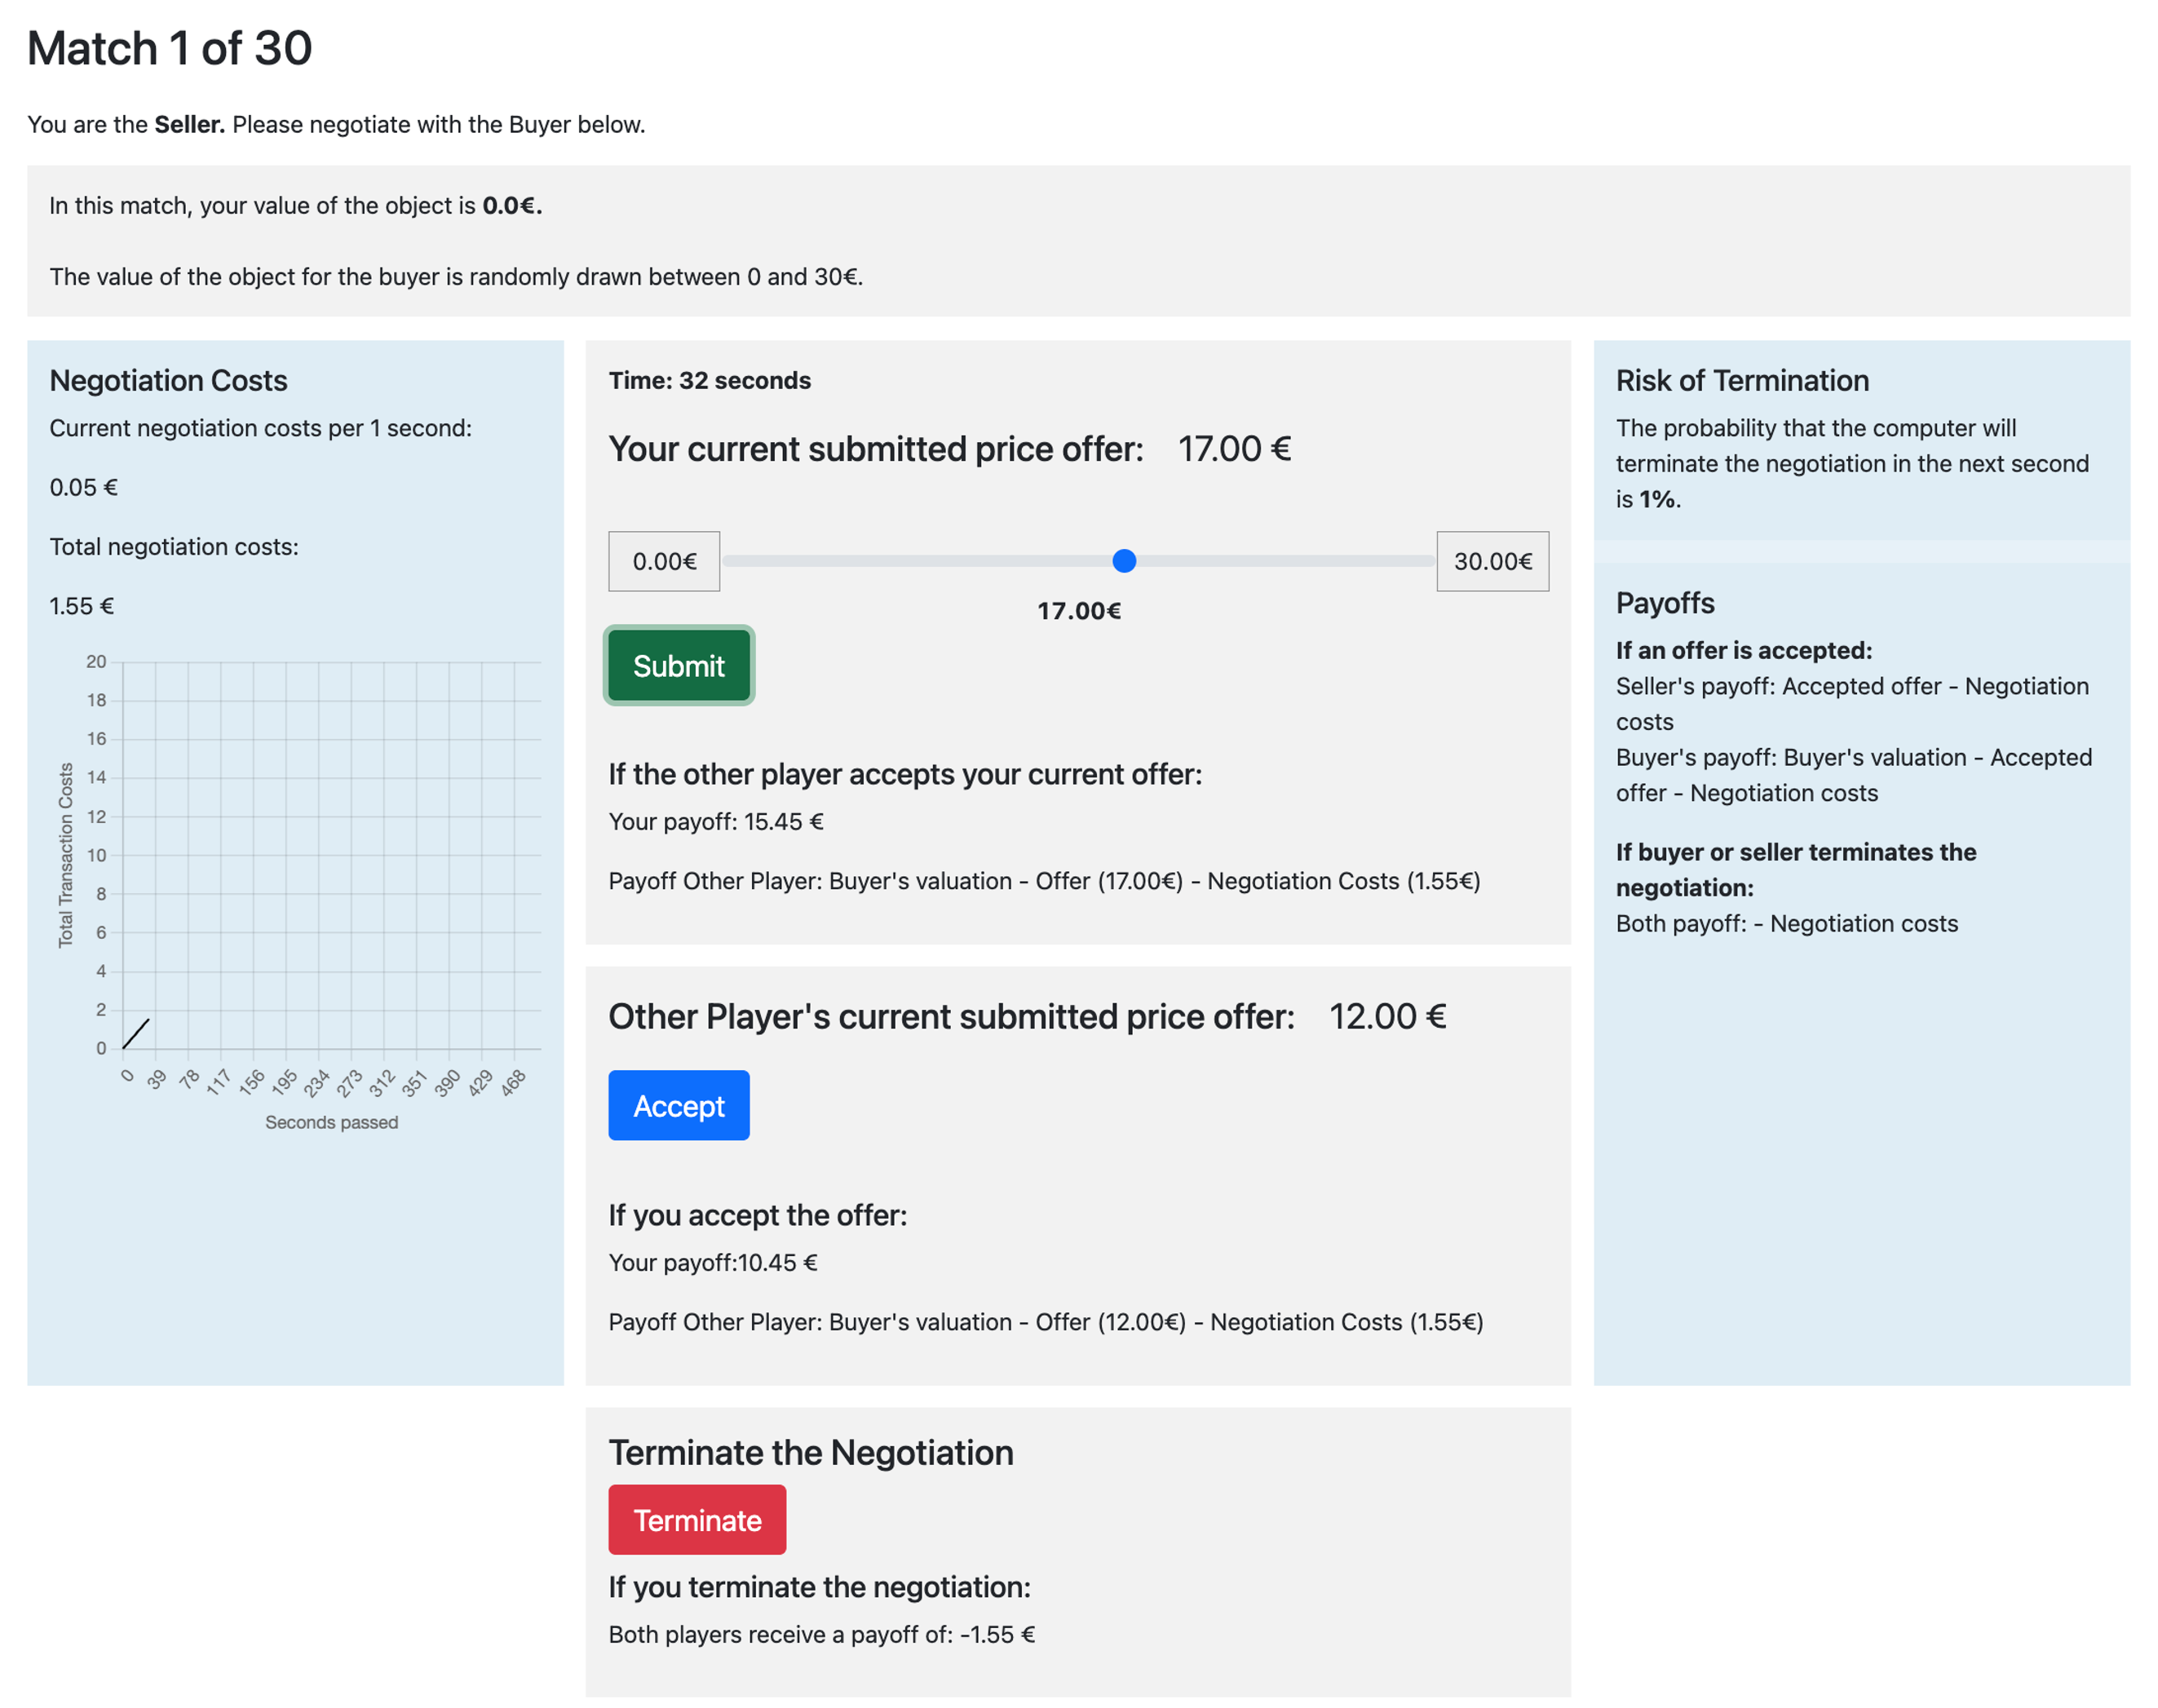
\includegraphics[width=0.8\linewidth]{figures/manual_figures/figure_seller.png}
    \caption{Bargaining Environment for Seller.}
    \label{fig:env_seller}
\end{figure}

In this environment, we automatically calculate payoffs for the participant for her current submitted offer, in case she accepts the other player's offer or in case of termination to reduce cognitive burden in the decision-making process. We also help participants to reduce mistakes when submitting an offer: In case buyers attempt to make an offer above their valuation (or sellers make an offer below their valuation), they are shown a pop-up window, asking them if they are sure to make this offer. 




%----------------------------------------------------------------
\subsection{Hypotheses}\label{subsec:hypotheses}
%----------------------------------------------------------------
Our model in \Fref{sec:model} and related models deliver predictions for some of the cells in our \(2\times2\) laboratory design.  The first group our hypotheses follow directly from these equilibrium models and are on which trades occur, how quickly, and at what terms.  The second group is more ad-hoc and exploratory 
and is derived from related empirical as well as theoretical papers.
%----------------------------------------------------------------
\paragraph{Theory–driven predictions.}
%----------------------------------------------------------------
In treatment T4 (\textit{Costly, Buyer-only Uncertainty}) our model yields a “three‐region” equilibrium. Calibrating our model to the values in the experimental environment, buyers with a valuation below \(b^{\dagger}=7.72\) should terminate immediately; those with \(b^{\dagger}<b<b^{*}=21.40\) should wait and eventually transact at \(p=b/2\); and buyers with \(b\ge b^{*}\) should accept the seller’s opening price \(p=b^{*}/2\) on the spot.  

In the treatments where only the sellers valuation is public (T3 and T4), the seller has no strategic reason to delay her offer; our model predicts she is more likely to make the first offer. 

We do not have precise theoretical predictions for the cases where both valuations are private (T1 and T2). However, we conjecture that the qualitative predictions align with \citet{cramton_strategic_1992} who studies the same model but without transaction costs. Sellers and buyers initially remain silent to signal their private information to the other side. A buyer with a high valuation (respectively, a seller with a low valuation) breaks the silence earlier than others, as they have a large surplus to loose and delay is thus more costly for them. After one party gives a signal about her type by breaking the silence, bargaining unfolds similarly to the case with one-sided asymmetric information. \textcolor{red}{We also predict a first-mover advantage in these settings based on \citep{rubinstein1982perfect}; the player who makes the first move extracts a larger part of the surplus}. \\

Finally, with regards to our main comparative static---the introduction of negotiation costs---our model predicts more terminations, shorter bargaining durations, less offers and lower efficiency (defined as the share of negotiations not ending in agreement although the surplus positive). 

To summarize, our five main hypotheses are:
\begin{enumerate}[label=\textbf{H\arabic*},leftmargin=1.4cm]
  \item \textbf{Threshold equilibrium}.  
        In T4 (\textit{Costly, Buyer-only Uncertainty}) the empirical distributions of prices and
        agreement times should exhibit the two theoretical cut‐offs
        \(b^{\dagger}\) and \(b^{*}\).
  \item \textbf{Seller first‐mover}.  
        In the two one‐sided uncertainty treatments (T3 and T4), the seller is more likely to make the first offer.
 \item \textbf{First‐mover advantage}.  
        In the two-sided uncertain information treatments (T1 and T2), the player with the first offer can extract a larger part of the surplus.
  \item \textbf{Silent signaling}.  
        Under two‐sided uncertainty, longer silence signals a lower valuation. 
  \item \textbf{Transaction‐cost effect}.  
        Adding the per‐second transaction cost is expected to (a) Reduce the number of offers,
        (b) shorten median bargaining duration, and (c) lower the efficiency
        loss relative to the first–best benchmark (successful trade in case of positive surplus).
\end{enumerate}

%----------------------------------------------------------------
\paragraph{Exploratory predictions.}
%----------------------------------------------------------------
Although our model is silent about behavioural heterogeneity, the experimental
literature points to a set of regularities that we will examine.  The list
below is necessarily selective; its purpose is to organise the ancillary
analysis rather than to exhaust all possible behavioural dimensions. The predictions are mostly based on \citet{bochet_beyond_2024}.

\begin{enumerate}[label=\textbf{E\arabic*},leftmargin=1.4cm]
  \item \textbf{Risk tolerance}.  More risk‐tolerant pairs should settle faster
        and reach agreement more often.
  \item \textbf{Fairness}.  Stronger distributive preferences
        lower efficiency.
  \item \textbf{Demand curvature}.  Acceptance rates should be highest for offers around a 50–50 surplus split and fall as offers move away from the midpoint.
  \item \textbf{Counter‐offers}.  A bid that responds to a previous offer is
        more likely to be accepted than an opening bid of the same magnitude.
  \item \textbf{Split‐the‐difference}.  Offers that halve the
        bid–ask gap have above‐average acceptance rates.
  \item \textbf{Learning}.  Agreement rates and efficiency are expected to rise
        over rounds as subjects gain experience.
  \item \textbf{Deadline memory}.  Negotiations that follow immediately after a
        computer‐terminated round should conclude faster; the effect is
        expected to fade within a few rounds \citep{enke2024associative}.
\end{enumerate}






\begin{comment}
    

\subsection{Hypotheses}

Our hypotheses are guided from our model presented in \Fref{sec:model}.

For the one-sided uncertainty case with transaction costs, our equlibrium prediction is:
Hypothsis 1: Equilibrium Payoffs: We define two thresholds: one is 21.4, and the other is 7.72. (1) Buyers with a value higher than 21.4 trade immediately at a price that is half of the higher threshold. Their payoff is their value minus half the higher threshold. (1) Buyers with a value below 7.72 exit immediately and get zero. (3) Buyers with a value between 7.72 and 21.4 trade after some delay, at a price equal to half their value. Their expected payoff is their value adjusted for the discount rate and transaction cost. 
In our case, the seller's valuation is public information, so her offer timing cannot signal any additional information. 
Hypothesis 2: Sellers make the first offer in the one-sided incomplete information case. 


Our design withwith two-sided asymmetric information is exploratory, and we do not yet have precise theoretical predictions yet. However, we conjecture that the qualitative predictions align with \citet{cramton_strategic_1992}, who studies the same model but without transaction costs. Here is the theoretical prediction for that model: Sellers and buyers initially remain silent to signal their private information to the other side. A buyer with a high valuation (respectively, a seller with a low valuation) breaks the silence earlier than others, as delay is more costly for them. After one party reveals their type by breaking the silence, the bargaining unfolds similarly to the case with one-sided asymmetric information. The person with the first offer is at an advantage and extracts on average a higher surplus (based on \citet{rubinstein1982perfect}). 

Comparing one-sided to two-sided uncertainty, we conjecture that higher uncertainty leads to less efficient outcomes \citep{myerson1983efficient, chatterjee1987bargaining}. Intuitively, both parties may suffer efficiency losses, but each tries to extract a greater share by appearing ``tough'', leading to an inefficiently slow convergence. Also, we now hypothesize that sellers can extract a greater amount of the suprlus in the two-sided asymettry case since they are not at a disadvantage anymore as now both players have private information. 

Our main comparative static is reaction to transaction costs. We hpothesize that bargaining without transaction csots leads to less terminations, longer bargaining durationas, more offers and more efficiency (as measured by successful transactions where surplus is positive). 

Derived from the literature, we also test the following exploratory hypotheses about the bargaining process which arises endogenously derived from \citep{bochet_beyond_2024}:

\begin{itemize}
    \item Higher risk tolerance of agents leads to higher efficiency 
    \item If people have a weaker fairness preferences, efficiency is higher 
    \item We add a quadratic term to predict offer acceptance as a fucntion of the demanded surplus share, hypothesizing that the more the demand deviates from a 50-50 split, the lower likelihood of acceptance
    \item Counteroffers are more likely to be accepted
    \item Split the difference offers are more likely to be accepted
    \item Efficiency gets larger as negotiators get more experienced
    \item There is a memory effect: In negotiations immediately after computer termination, agents negotiate faster; however this effect fades over time \citep{enke2024associative}
\end{itemize}




\end{comment}






\section{Main Results}
\label{sec:main_results}



\subsection{Buyer-Only Uncertainty}

\paragraph{H1 Threshhold Equilibrium}




\subsection{Symmetric Uncertainty}

\label{sec:conclusion}



\newpage 

\bibliographystyle{aer}
\bibliography{references} 

\newpage

\begin{appendices}
\begin{center}
 {\Large Online Appendix\\ {\bf Time and Informtion in Bargaining}}\\[1.25cm]
    
    {\large ... \hspace{1cm}
   ...\hspace{1cm}\\
    ...\hspace{1cm}    
    Nicolas R\"over}\\[1.25cm]
    
    {\large \today}\\[1.25cm]
\end{center}
\newpage




\section{Figures}




\begin{figure}
     \centering
     \begin{subfigure}[h]{0.65\textwidth}
         \centering
         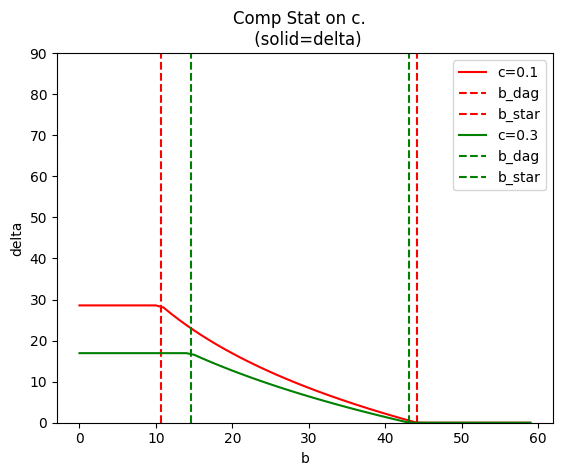
\includegraphics[width=\textwidth]{./fig/fig_01_a.png}
         \caption{$r=0.04$}
     \end{subfigure}
     \hfill

     \bigskip
     \begin{subfigure}[h]{0.65\textwidth}
         \centering
         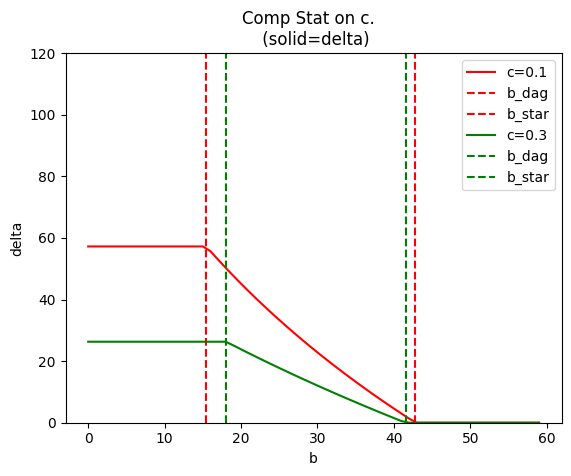
\includegraphics[width=\textwidth]{./fig/fig_01_b.png}
         \caption{$r= 0.01$}
     \end{subfigure}
     \caption{Vertical axis = $\Delta(b;b^*)$= (agreement time). Vertical dashed lines = $b^*$ and $b^\dagger$.
    The buyer types lower than $b^\dagger$ terminate at $t=0$. Hence, the ``flat'' parts of the graphs over the range $[0,b^\dagger]$ should be disregarded. The same comment applies to the next figure.
    }
    \label{f:01}
\end{figure}

\phantom{a}

\begin{figure}
     \centering
     \begin{subfigure}[h]{0.65\textwidth}
         \centering
         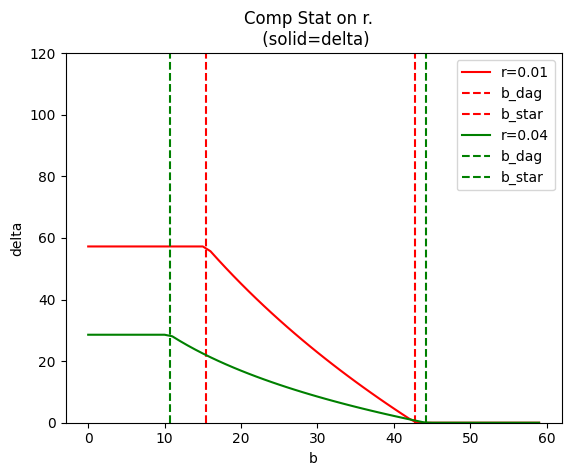
\includegraphics[width=\textwidth]{./fig/fig_02_a.png}
         \caption{$c=0.10$}
     \end{subfigure}
     \hfill

     \bigskip
     \begin{subfigure}[h]{0.65\textwidth}
         \centering
         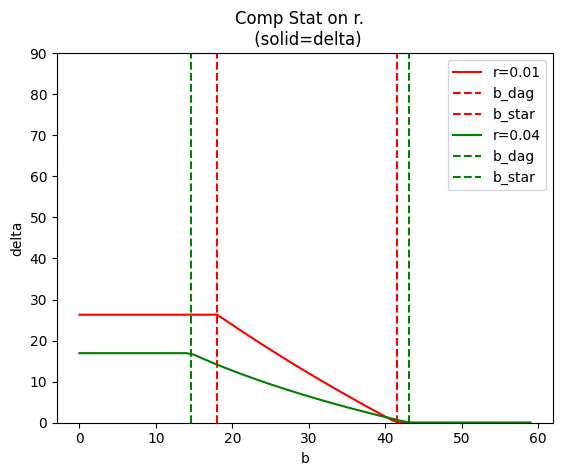
\includegraphics[width=\textwidth]{./fig/fig_02_b.png}
         \caption{$c=0.30$}
     \end{subfigure}
     \caption{Vertical axis = $\Delta(b;b^*)$ = (agreement time). Vertical dashed lines = $b^*$ and $b^\dagger$.}
     \label{f:02}
\end{figure}

\phantom{a}

\begin{figure}
     \centering
     \begin{subfigure}[h]{0.65\textwidth}
         \centering
         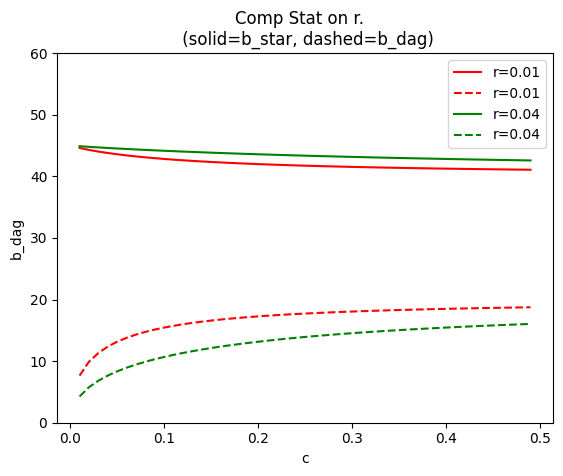
\includegraphics[width=\textwidth]{./fig/fig_03_a.png}
     \end{subfigure}
     \hfill
     
     \bigskip 
     \begin{subfigure}[h]{0.65\textwidth}
         \centering
         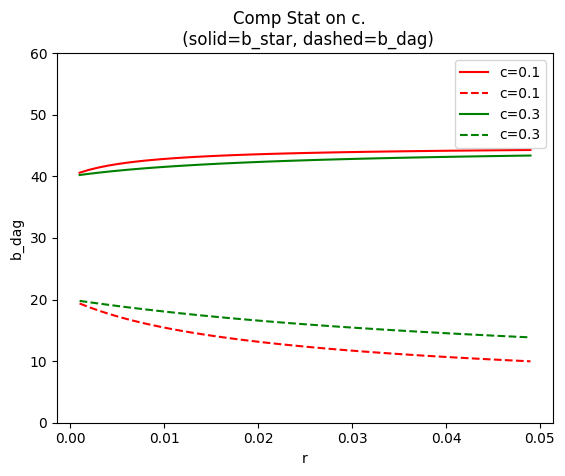
\includegraphics[width=\textwidth]{./fig/fig_03_b.png}
     \end{subfigure}
     \caption{Vertical Axis = $b^*$ and $b^\dagger$.}
\end{figure}


\phantom{a}

\begin{figure}
     \centering
     \begin{subfigure}[h]{0.65\textwidth}
         \centering
         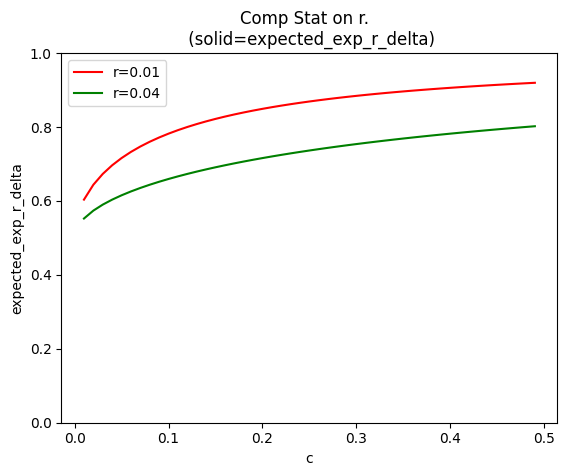
\includegraphics[width=\textwidth]{./fig/fig_04_a.png}
%        \caption{Green: Weekly payment. Red: Daily payment.}
     \end{subfigure}
     \hfill

     \bigskip
     \begin{subfigure}[h]{0.65\textwidth}
         \centering
         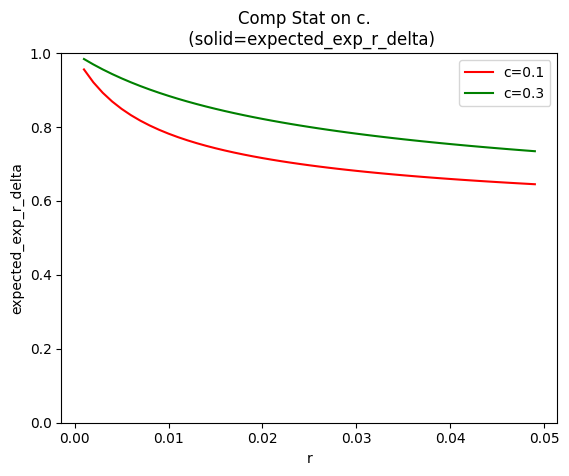
\includegraphics[width=\textwidth]{./fig/fig_04_b.png}
%         \caption{Green: $c=0.75$. Red: $c=0.25$.}
     \end{subfigure}
     \caption{Vertical Axis = $\mathbbm{E}[e^{-r\Delta(b|b^*)}|b\in\mathcal{I}(b,c)]$.}
\end{figure}

\section{Proofs of Propositions \ref{p:uniform_symmetric_cs_c} and \ref{p:uniform_symmetric_cs_r}}

\paragraph{Proof of Proposition \ref{p:uniform_symmetric_cs_c}.}
We prove the proposition by proving four claims in sequence. 

\begin{claim}\label{claim:uniform_symmetric_cs_kappa:01}
$b^*$ decreases as $\kappa=c/r$ increases. 
\end{claim}

\begin{proof}[Proof of Claim \ref{claim:uniform_symmetric_cs_kappa:01}]
It suffices to show that 
    $$
    \frac{\partial^2\Pi_S(b)}{\partial b\partial \kappa} 
    =
    \frac{\partial^2}{\partial b\partial \kappa}\left[\frac{(\overline b-b)(b-s)}{2} + \frac{Y(b)^2-6\kappa Y(b)+4\kappa\sqrt{2\kappa Y(b)}}{6}\right]<0. 
    $$
Note that
    \begin{align*}
    &\frac{\partial^2}{\partial b\partial \kappa} [Y(b)^2] 
    = \frac{\partial}{\partial \kappa}[2Y(b)]=
    4
    \quad\text{and}\quad
    \frac{\partial^2}{\partial b\partial \kappa} [6\kappa Y(b)]
    =\frac{\partial}{\partial \kappa}[6\kappa] = 6. 
    \end{align*}
Furthermore,
    \begin{align*}
    \frac{\partial^2}{\partial b\partial \kappa}
    [4\kappa\sqrt{2\kappa Y(b)}]
    &=\frac{\partial}{\partial \kappa}[ (2\kappa)^{3/2} Y(b)^{-1/2}]
    = 3 \left[\frac{2\kappa}{Y(b)}\right]^{1/2}- \left[\frac{2\kappa}{Y(b)}\right]^{3/2}<2
    \end{align*}
where the last inequality holds because $3y^{1/2}- y^{3/2}< 2$ for all $y\in(0,1)$. Thus,
    \begin{align*}
    \frac{\partial^2\Pi_S(b)}{\partial b\partial \kappa} 
    &
    < \frac{4-6+2}{6} =0.
    \end{align*}
Then, the monotonicity of $b^*$ with respect to $\kappa$ follows the standard comparative statics argument. 
\end{proof}


Does $b^\dagger(\kappa)$ increase or decrease in $c$? 
Choose $\kappa_L$ and $\kappa_H$ such that $0<\kappa_L<\kappa_H$ and, furthermore, both $(b^\dagger(\kappa_L), b^*(\kappa_L))$ and $(b^\dagger(\kappa_H), b^*(\kappa_H))$ are non-empty. 
We will consider what happens to the buyer type $b^\dagger(\kappa_L)$ as $c$ increases from $c_L=\kappa_L r $ to $c_H=\kappa_H r$. There are two countervailing effects of such an increase of $c$.
    \begin{itemize}
    \item Consider the case such that $c=c_L$. In equilibrium, the buyer type $b=b^\dagger(\kappa_L)$ delays the negotiation to distinguish herself from other buyer types in $(b^\dagger(\kappa_L),b^*(\kappa_L))$. $b^*(\kappa)$ decreases as $c$ increases from $c_L$ to $c_H$, and thus, there would be \emph{fewer} buyer types less than $b^*$. Thus, the buyer type $b^\dagger
(\kappa_L)$ needs to delay by a \emph{shorter} amount of time. This effect increases the payoff of $b^\dagger(\kappa_L)$ from delaying. 

    \item However, as $c$ increases from $c_L$ to $c_H$, the total negotiation cost increases, \emph{conditional on} the duration of delay being fixed. This effect decreases the payoff of $b=b^\dagger(\kappa_L)$ from delaying.
     
    \end{itemize}
It is unclear which effect dominates. As a result, it is intuitively not clear whether $b^\dagger(\kappa)$ decreases or increases in $\kappa$. 
\bigskip


\begin{claim}\label{claim:uniform_symmetric_cs_c:02} Fix $r>0$ and consider $c_L$ and $c_H$ such that both $0<c_L<c_H$. Then, 
    $$
    \Delta(b;b^*(c_L,r)) > \Delta(b;b^*(c_H,r)) \quad\forall b\in \mathcal{I}(c_L,r)\cap \mathcal{I}(c_H,r). 
    $$
\end{claim}

\begin{proof}[Proof of Claim \ref{claim:uniform_symmetric_cs_c:02}] 
Note that 
    $$
    \Delta(b|b^*(c,r)) = \frac{1}{r}\log\frac{b^*(\kappa)-s+2(c/r)}{b-s+2(c/r)}.
    $$
By Claim \ref{claim:uniform_symmetric_cs_kappa:01}, $\partial b^*(c,r)/\partial c<0$. Thus, 
    \begin{align*}
    &
    \frac{\partial \log (b-s+2(c/r))}{\partial c}=
    \frac{d\log (b-s+2\kappa)}{d \kappa}\frac{1}{r} = \frac{2}{b-s+2(c/r)} \frac{1}{r}.
    \end{align*}
Similarly, 
    \begin{align*}
    \frac{\partial\log (b^*(c,r)-s+2(c/r))}{\partial c} = \frac{\partial b^*/\partial c+2}{b^*-s+2(c/r)}\frac{1}{r}
    \leq  \frac{2}{b^*-s+2(c/r)}\frac{1}{r} < \frac{2}{b-s+2(c/r)}\frac{1}{r}
    \end{align*}
where the first inequality holds because $b^*$ decreases in $c$; the second inequality holds because $b^*>b$. Thus, $\Delta(b;b^*(c,r))$ decreases in $c$.
\end{proof}




\begin{claim}\label{claim:uniform_symmetric_cs_c:03} 
Fix $r>0$, $c_L$, and $c_H$ such that $c_L<c_H$. Then, $\Delta(b^\dagger(c_L,r);b^*(c_L,r)) > \Delta(b^\dagger(c_H,r);b^*(c_H,r))$. Equivalently,
    $$
    e^{-r\Delta(b^\dagger(c_H,r);b^*(c_H,r))}> e^{-r\Delta(b^\dagger(c_L,r);b^*(c_L,r))}.
    $$
\end{claim}

\begin{proof}[Proof of Claim \ref{claim:uniform_symmetric_cs_c:03}]
First, consider the case $b^\dagger(c_L, r) \leq b^\dagger(c_H, r)$. In this case, 
    \begin{align*}
    -r\Delta(b^\dagger(c_H, r)|b^*(c_H, r))
    &=\log\frac{r(b^\dagger(c_H, r)-s)+2c_H}{r(b^*(c_H, r)-s)+2c_H}
    \\
    &> \log\frac{r(b^\dagger(c_H, r)-s)+2c_L}{r(b^*(c_H, r)-s)+2c_L} \;\because r(b^*(c_H, r)-s)> (b^\dagger(c_H, r)-s)
    \\
    &\geq \log\frac{r(b^\dagger(c_H, r)-s)+2c_L}{r(b^*(c_L, r)-s)+2c_L} \quad \because b^*(c_L, r) \geq b^*(c_H, r)
    \\
    &\geq \log\frac{r(b^\dagger(c_L, r)-s)+2c_L}{r(b^*(c_L, r)-s)+2c_L} = -r\Delta(b^\dagger(c_L, r)|b^*(c_L, r)). 
    \end{align*} 
Thus, $\Delta(b^\dagger(c_L, r);b^*(c_L, r)) > \Delta(b^\dagger(c_H, r);b^*(c_H, r))$ whenever $b^\dagger(c_L, r) \leq b^\dagger(c_H, r)$. 

Next, consider the case $b^\dagger(c_L, r) > b^\dagger(c_H, r)$. Suppose for contradiction 
    \begin{align*}
    &\Delta(b^\dagger(c_L, r);b^*(c_L, r)) \leq \Delta(b^\dagger(c_H, r);b^*(c_H, r)) 
    \\
    \iff&
    e^{-r\Delta(b^\dagger(c_L, r);b^*(c_L, r))} \geq e^{-r\Delta(b^\dagger(c_H, r);b^*(c_H, r))}.
    \end{align*}
But then, we obtain the following contradiction: 
    \begin{align*}
    0&=e^{-r\Delta(b^\dagger(c_L, r);b^*(c_L, r))}\left(b^\dagger(c_L, r)-p^R(b^\dagger(c_L, r),s)+\frac{c_L}{r}\right)-\frac{c_L}{r}
    \\
    &\geq e^{-r\Delta(b^\dagger(c_H, r);b^*(c_H, r))}\left(b^\dagger(c_L, r)-p^R(b^\dagger(c_L, r),s)+\frac{c_L}{r}\right)-\frac{c_L}{r}
    \\
    &> e^{-r\Delta(b^\dagger(c_H, r);b^*(c_H, r))}\left(b^\dagger(c_L, r)-p^R(b^\dagger(c_L, r),s)+\frac{c_H}{r}\right)-\frac{c_H}{r} 
    \\
    &\geq e^{-r\Delta(b^\dagger(c_H, r);b^*(c_H, r))}\left(b^\dagger(c_H, r)-p^R(b^\dagger(c_H, r),s)+\frac{c_H}{r}\right)-\frac{c_H}{r} \geq 0, 
    \end{align*}
where the last weak inequality follows the buyer's individual rationality. Note that the first equality holds because $b^\dagger(c_L, r) > b^\dagger(c_H, r)\geq\underline b\vee s$, and thus, the equilibrium payoff of $b=b^\dagger(c_L, r)$ must be zero. The last inequality may not hold as equality if we have $b^\dagger(c_H, r)=\underline b\vee s$. 
\end{proof}

\begin{claim}\label{claim:uniform_symmetric_cs_c:04} 
Fix $r>0$. $\mathbbm{E}[e^{-r\Delta(b;b^*(c,r))}|b\in \mathcal{I}(c,r)]$ increases in $c$ at any $c$ such that $\mathcal{I}(c,r)\neq\emptyset$. 
\end{claim}

\begin{proof}[Proof of Claim \ref{claim:uniform_symmetric_cs_c:04}] 
Note that
    $$
    e^{-r\Delta(b;b^*(c,r))}=\frac{r(b-s)+2c}{r(b^*(c,r)-s)+2c} \quad\forall b\in \mathcal{I}(c,r)
    $$
is linear in $b$. Hence, because $b$ is drawn from a uniform distribution, 
    \begin{align*}
    \mathbbm{E}[e^{-r\Delta(b;b^*(c,r))}|b\in \mathcal{I}(c,r)] 
    & = 
    \frac{1}{2}\left[e^{-r\Delta(b^*(c,r)|b^*(c,r))}+e^{-r\Delta(b^\dagger(c,r)|b^*(c,r))}\right]
    \\
    &=
    \frac{1}{2}\left[1+e^{-r\Delta(b^\dagger(c,r)|b^*(c,r))}\right]
    \end{align*}
where the last equality holds by construction. $e^{-r\Delta(b^\dagger(c,r)|b^*(c,r))}$ increases in $c$ (Claim \ref{claim:uniform_symmetric_cs_c:03}), and thus, the result is obtained. 
\end{proof}

\paragraph{Proof of Proposition \ref{p:uniform_symmetric_cs_r}.}
We prove the proposition by proving three claims in sequence. 

\begin{claim}\label{claim:uniform_symmetric_cs_r:05} 
Fix $c>0$ and consider $r_L$ and $r_H$ such that both $0<r_L<r_H$. Then, 
    $$
    r_L\Delta(b;b^*(c,r_L)) < r_H\Delta(b;b^*(c,r_H)) \quad\forall b\in \mathcal{I}(c,r_L)\cap \mathcal{I}(c,r_H). 
    $$
\end{claim}


\begin{proof}[Proof of Claim \ref{claim:uniform_symmetric_cs_r:05}] 
Note that 
    $$
    r\Delta(b|b^*) = \log\frac{b^*-s+2(c/r)}{b-s+2(c/r)}.
    $$
By Claim \ref{claim:uniform_symmetric_cs_kappa:01}, $\partial b^*(c,r)/\partial r>0$. Thus, 
    \begin{align*}
    &
    \frac{\partial \log (b-s+2(c/r))}{\partial r}=
    \frac{d\log (b-s+2\kappa)}{d \kappa}\left(-\frac{c}{r^2}\right) = \frac{2}{b-s+2(c/r)} \left(-\frac{c}{r^2}\right).
    \end{align*}
Similarly, 
    \begin{align*}
    \frac{\partial\log (b^*(c,r)-s+2(c/r))}{\partial r} = \frac{\partial b^*/\partial r-\frac{2c}{r^2}}{b^*-s+2(c/r)}
    &\geq  \frac{2}{b^*-s+2(c/r)}\left(-\frac{c}{r^2}\right)
    \\
    &> \frac{2}{b-s+2(c/r)}\left(-\frac{c}{r^2}\right)
    \end{align*}
where the first inequality holds because $b^*$ increases in $r$; the second inequality holds because $b^*>b$. Thus, $r\Delta(b;b^*(c,r))$ increases in $r$.
\end{proof}


\begin{claim}\label{claim:uniform_symmetric_cs_r:06}
Fix $c>0$, $r_L$, and $r_H$ such that $0<r_L<r_H$. Then, $r_L\Delta(b^\dagger(c,r_L);b^*(c,r_L)) < r_H\Delta(b^\dagger(c,r_H);b^*(c,r_H))$. Equivalently,
    $$
    e^{-r_L\Delta(b^\dagger(c,r_L);b^*(c,r_L))}> e^{-r_H\Delta(b^\dagger(c,r_H);b^*(c,r_H))}.
    $$
\end{claim}

\begin{proof}[Proof of Claim \ref{claim:uniform_symmetric_cs_r:06}]
First, consider the case $b^\dagger(c, r_L) \geq b^\dagger(c, r_H)$. In this case, 
    \begin{align*}
    -r_L\Delta(b^\dagger(c, r_L)|b^*(c, r_L))&=\log\frac{r_L(b^\dagger(c, r_L)-s)+2c}{r_L(b^*(c, r_L)-s)+2c}
    \\
    &\geq \log\frac{r_L(b^\dagger(c, r_H)-s)+2c}{r_L(b^*(c, r_H)-s)+2c} \quad \because b^*(c, r_L) \leq b^*(c, r_H)
    \\
    &> \log\frac{r_H(b^\dagger(c, r_H)-s)+2c}{r_H(b^*(c, r_H)-s)+2c} = -r_H\Delta(b^\dagger(c, r_H)|b^*(c, r_H)). 
    \end{align*} 
   where the 
Thus, $r_L\Delta(b^\dagger(c, r_L);b^*(c, r_L)) < r_H\Delta(b^\dagger(c, r_H);b^*(c, r_H))$ whenever $b^\dagger(c, r_L) \geq b^\dagger(c, r_H)$. 
Next, consider the case $b^\dagger(c, r_L) < b^\dagger(c, r_H)$. Suppose for contradiction 
    \begin{align*}
    &r_L\Delta(b^\dagger(c, r_L);b^*(c, r_L)) \geq r_H\Delta(b^\dagger(c, r_H);b^*(c, r_H)) 
    \\
    \iff&
    e^{-r_L\Delta(b^\dagger(c, r_L);b^*(c, r_L))} \leq e^{-r_H\Delta(b^\dagger(c, r_H);b^*(c, r_H))}.
    \end{align*}
But then, we obtain the following contradiction: 
    \begin{align*}
    0&=e^{-r_H\Delta(b^\dagger(c, r_H);b^*(c, r_H))}\left(b^\dagger(c, r_H)-p^R(b^\dagger(c, r_H),s)+\frac{c}{r_H}\right)-\frac{c}{r_H}
    \\
    &\geq e^{-r_L\Delta(b^\dagger(c, r_L);b^*(c, r_L))}\left(b^\dagger(c, r_H)-p^R(b^\dagger(c, r_H),s)+\frac{c}{r_H}\right)-\frac{c}{r_H}
    \\
    &>e^{-r_L\Delta(b^\dagger(c, r_L);b^*(c, r_L))}\left(b^\dagger(c, r_L)-p^R(b^\dagger(c, r_L),s)+\frac{c}{r_H}\right)-\frac{c}{r_H}
    \\
    &>e^{-r_L\Delta(b^\dagger(c, r_L);b^*(c, r_L))}\left(b^\dagger(c, r_L)-p^R(b^\dagger(c, r_L),s)+\frac{c}{r_L}\right)-\frac{c}{r_L} \geq 0, 
    \end{align*}
where the last weak inequality follows the buyer's individual rationality. 
\end{proof}

\begin{claim}\label{claim:uniform_symmetric_cs_r:07} 
Fix $c>0$. $\mathbbm{E}[e^{-r\Delta(b;b^*(c,r))}|b\in \mathcal{I}(c,r)]$ decreases in $r$ at any $r$ such that $\mathcal{I}(c,r)\neq\emptyset$. 
\end{claim}

\begin{proof}[Proof of Claim \ref{claim:uniform_symmetric_cs_r:07}] 
Note that
    $$
    e^{-r\Delta(b;b^*(c,r))}=\frac{r(b-s)+2c}{r(b^*(c,r)-s)+2c} \quad\forall b\in \mathcal{I}(c,r)
    $$
is linear in $b$. Hence, because $b$ is drawn from a uniform distribution, 
    \begin{align*}
    \mathbbm{E}[e^{-r\Delta(b;b^*(c,r))}|b\in \mathcal{I}(c,r)] 
    & = 
    \frac{1}{2}\left[e^{-r\Delta(b^*(c,r)|b^*(c,r))}+e^{-r\Delta(b^\dagger(c,r)|b^*(c,r))}\right]
    \\
    &=
    \frac{1}{2}\left[1+e^{-r\Delta(b^\dagger(c,r)|b^*(c,r))}\right]
    \end{align*}
where the last equality holds by construction. $e^{-r\Delta(b^\dagger(c,r)|b^*(c,r))}$ decreases in $r$ (Claim \ref{claim:uniform_symmetric_cs_r:06}), and thus, the result is obtained. 
\end{proof}



\end{appendices}
\end{document}
